\documentclass[11pt, a4paper, lithuanian]{article}

\usepackage[left=25mm,right=15mm,top=15mm,bottom=15mm]{geometry}
\usepackage[utf8x]{inputenc}
\usepackage[L7x]{fontenc}
\usepackage[lithuanian]{babel}
\usepackage{listings}
\usepackage{amsmath, amssymb}
\usepackage{graphicx}
 \usepackage{url}

\author{AKSfm-15, Maksim Norkin}
\title{Vaizdo atpažinimas}

\lstset{
  language=Matlab,
  basicstyle=\footnotesize,
  columns=fixed,
  numbers=none,
  showspaces=false,
  xleftmargin=20pt
}

\begin{document}

    \maketitle

    \section{Užduotis}

    Naudodami savo sukurtas arba specializuotas MATLAB funkcijas, atpažinkite vaizde pateiktus ranka rašytus skaičius. Vaizdo apdorojimui galite pasinaudoti jau sukurtomis funkcijomis (vaizdo segmentavimo, vienodo, 50x70 taškų, dydžio kvadratėlių su skaičiais paruošimo, 35 požymių išskyrimo...). Galite paruošti savo vaizdus ir požymiams išskirti naudoti šią funkciją (reikia nurodyti paveikslėlio pavadinimą ir simbolių eilučių vaizde skaičių).

    \section{Vaizdo atpažinimas}

    Pirminis žingsnis vaizdo apdorojime yra vaizdo paruošimas apdorojimui. Turimas vaizdas yra trijų dimensijų, RGB, todėl pirmiausiai reikia sumažinti kanalų skaičių iki vieno. Tai yra atliekama Matlab \textit{im2bw} funkcijos pagalba, kaip parodyta \ref{code:pradinio_vaizdo_paruosimas} pav.

    \begin{figure}[h]
      \centering
      \caption{Pradinio vaizdo paruošimas}
      \label{code:pradinio_vaizdo_paruosimas}
      \begin{lstlisting}
I = imread('skaiciai.bmp');

I = im2bw(I, 0.86);
      \end{lstlisting}
    \end{figure}

    Sekantis žingsnis yra vaizdo segmentavimas. Reikalinga pilnai izoliuoti vaizdo dalis ir pašalinti foninį vaizdą. Tai yra pasiekiama panaudojus briaunos detektavimo algoritmą ir dviejų dimensijų filtrą, kurio paskirtis yra užpildyti susidariusias ``skyles'' vaizde. Toliau panaudojam regionų savybių Matlab funkcija, tam kad sužinoti nagrinėjamo vaizdo segmento centrą, \ref{code:vaizdo_segmentavimas} pav.

    \begin{figure}[h]
      \centering
      \caption{Vaizdo segmentavimas}
      \label{code:vaizdo_segmentavimas}
      \begin{lstlisting}
% Full blown canny detection
I_e = edge(I, 'canny', [0.15 0.4]);

% Bluring everything for better region detection
I_f = imfilter(I_e, magic(5));

% Go for areal statistics
stats = regionprops(I_f, 'BoundingBox', 'Area');
      \end{lstlisting}
    \end{figure}

    Taip mes gauname 50 ilgio vektorių, kur kas 5 elementas yra sekantis skaičius vaizde. Toliau seka vaizdo elementų subendrinimas į $32x32$ dydžio matricas, \ref{code:vaizdo_paruosimas_klasifikavimui} pav.

    \begin{figure}[h]
      \centering
      \caption{Vaizdo paruošimas klasifikavimui}
      \label{code:vaizdo_paruosimas_klasifikavimui}
      \begin{lstlisting}
NNs = {};

for k=1:length(stats)
    bb = round(stats(k).BoundingBox);
   
    I_c = I(bb(2):bb(2)+bb(4),bb(1):bb(1)+bb(3),:);
    NN{k} = imresize(I_c, [32 32]);
end
      \end{lstlisting}
    \end{figure}

    Sekantis žingsnis yra klasifikavimo mokymo ir tikrinimo elementų grupių sudarymas. Pirmiausiai reikia duomenis performuoti patogumui, kur pirma dimensija būtų nagrinėjamas skaičius (10 šiuo atveju yra 0), antra dimensija būtų pavyzdžio numeris ir galiausiai pats pavyzdys, performuotas iš matricos į vienos dimensijos vektorių, bendram patogumui, \ref{code:vaizdo_elementu_performavimas} pav.

    \begin{figure}[h]
      \centering
      \caption{Vaizdo elementų performavimas}
      \label{code:vaizdo_elementu_performavimas}
      \begin{lstlisting}
for k=1:5
    X(1,k,:) = reshape(NN{k}, [], 1);
    X(2,k,:) = reshape(NN{k+5}, [], 1);
    X(3,k,:) = reshape(NN{k+10}, [], 1);
    X(4,k,:) = reshape(NN{k+15}, [], 1);
    X(5,k,:) = reshape(NN{k+20}, [], 1);
    X(6,k,:) = reshape(NN{k+25}, [], 1);
    X(7,k,:) = reshape(NN{k+30}, [], 1);
    X(8,k,:) = reshape(NN{k+35}, [], 1);
    X(9,k,:) = reshape(NN{k+40}, [], 1);
    X(10,k,:) = reshape(NN{k+45}, [], 1);
end
      \end{lstlisting}
    \end{figure}

    Sudarome mokymo pavyzdžius, pasirinkdami pirmus tris pavyzdžius mokymui iš kiekvieno skaičiaus sekos, o tikrinimui likusius du. Tokiu stiliumi sudarome žymeklio vektorių, kuris skirtas klasifikavimo rezultatui tikrinti, \ref{code:mokymo_pavyzdziu_rinkinio_sudarymas} pav.

    \begin{figure}[h]
      \centering
      \caption{Mokymo pavyzdžių rinkinio sudarymas}
      \label{code:mokymo_pavyzdziu_rinkinio_sudarymas}
      \begin{lstlisting}
X_train = [
    X(1,1,:) X(1,2,:) X(1,3,:)
    X(2,1,:) X(2,2,:) X(2,3,:)
    X(3,1,:) X(3,2,:) X(3,3,:)
    X(4,1,:) X(4,2,:) X(4,3,:)
    % ir t.t.
];

X_predict = [
    X(1,4,:) X(1,5,:)
    X(2,4,:) X(2,5,:)
    % ir t.t.
];

X_train = double(reshape(X_train, [], 1024));
X_predict = double(reshape(X_predict, [], 1024));

Y_train = [1,1,1,2,2,2,3,3,3,4,4,4,5,5,5,6,6,6,7,7,7,8,8,8,9,9,9,0,0,0];
Y_predict = [1,1,2,2,3,3,4,4,5,5,6,6,7,7,8,8,9,9,0,0];

      \end{lstlisting}
    \end{figure}

    Po duomenų paruošimo sekantis žingsnis yra duomenų pateikimas mokymo algoritmui. Mokymo algoritmas parenkamas pasirinkimo medis, dėl gerų rezultatų pateikimo \cite{matlabexample}. Iškarto po mokymo galim atlikti likusių pavyzdžių klasifikavimą, \ref{code:klasifikatoriaus_mokymas} pav.

    \begin{figure}[h]
      \centering
      \caption{Klasifikatoriaus mokymas ir testuojamų duomenų atpažinimas}
      \label{code:klasifikatoriaus_mokymas}
      \begin{lstlisting}
mdl_tree = fitensemble(X_train,Y_train, 'Bag', 300, 'Tree', 'type', 'Classification');

Y_tree = predict(mdl_tree, X_predict);

      \end{lstlisting}
    \end{figure}

    Tokiu būdu yra gaunamas klasifikavimo rezultatas, \ref{fig:klasifikavimo_pasirinkimo_medziu_rezultatas} pav. Iš pateikto rezultato galima pastebėti, kad algoritmas blogai klasifikuoja du skaičius -- devynis ir aštuonis. Kitus skaičius algoritmas atpažino sėkmingai.

    \begin{figure}[h]
        \centering
        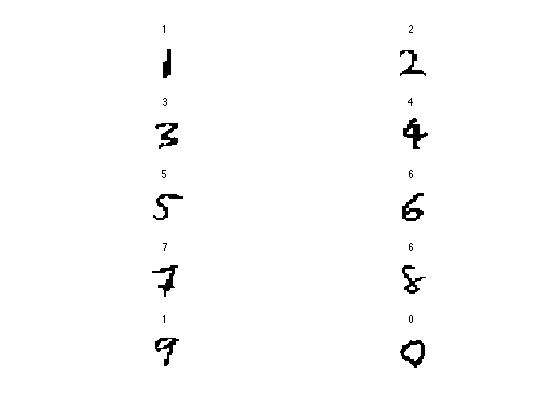
\includegraphics[width=300px]{img/rezultatas.jpg}
        \caption{Klasifikavimo pasirinkimo medžiu rezultatas}
        \label{fig:klasifikavimo_pasirinkimo_medziu_rezultatas}
    \end{figure}

    \section{Išvados}

    Laboratorinio darbo metu buvo sukurta Matlab programa, kuri atpažįsta vaizde pateiktus ranka rašytus skaičius. Vaizdo paruošimui buvo panaudotas vaizdo segmentavimas, panaudojus ``canny'' briaunos detektavimo algoritmą. Jo darbui pagerinti buvo panaudotas paprastas dviejų dimensijų binarinis filtras pirminiam vaizdui sutankinti. Sutankintas vaizdas toliau buvo izoliuotas į atskiras sekcijas iš originalaus vaizdo ir taip paruošti duomeny vaizdo klasifikavimui. Klasifikavimui parinktas medžio pasirinkimo klasifikatorius su $300$ elementų. Toks skaičius parinktas tik iš eksperimentinės pusės, didinant elementų skaičių ir stebinti klasifikavimo rezultatą. Iš klasifikavimo rezultato galima spręsti, jog klasifikatorius atliko blogą darbą ir sėkmingai neatpažino dviejų skaičių iš dešimties.

    \bibliographystyle{plain}
    \bibliography{references}


\end{document}